% !TEX root = ../Robotik.tex
\chapter{Schwarmrobotik und Evolutionäre Robotik}
Bei der Schwarmrobotik werden simple Roboter eingesetzt. Diese haben einzeln
nur ein sehr begrenzte Handlungs- und Wahrnehmungsmöglichkeiten. In der
Gemeinschaft agieren sie als intelligentes System.

\paragraph{Vorteil:} robust, skalierbar und flexibel
\begin{itemize}
	\item robust, skalierbar und flexibel
	\item \textbf{Kosten:} die einzelnen Roboter sind jeweils billig und können
		leichter ersetzt werden, als ein einzelner Großer.
	\item \textbf{Verlässlichkeit:} Ausfall eines einzelnen hat keine großen
		Auswirkungen $\Rightarrow$ Neustrukturierung und Koordination
	\item \textbf{Flexibilität:} Durch unterschiedliche Kooperation können die
		Roboter unterschiedlichste Aufgaben ausführen.
\end{itemize}

\textbf{Nachteil:} Schwarmverhalten nur schwer vorhersagbar

\section{Schwärme  und deren Verhalten in der Natur}
\paragraph{Schwarmdefinition}
Der Begriff \textbf{Schwarm} bezeichnet einen Verband von fliegenden oder
schwimmenden Lebewesen, der sich koordiniert bewegt. Im Unterschied zu anderen
Gruppen zeigt er ein sogenanntens \textbf{Schwarmverhalten}

\subsection{Computersimulation von Schwärmen - Algorithmus von Craig Reynolds}
Die einzelnen Individuen agieren in Abhängigkeit von der Position und der
Geschwindigkeit der benachbarten Boids nach folgenden Regeln:
\begin{description}
	\item[Separation] Bewege dich weg sobald dir andere zu nahe kommen
	\item[Alignment] Bewege dich in die gleiche Richtung wie deine Nachbarn
	\item[Cohesion] Bewege dich zum Mittelpunkt der Nachbarn
\end{description}

\paragraph{Vorraussetzung}
Reynolds setzte vorraus, dass \textbf{alle} Vögel innerhalb eines fixen
gegebenen Radius interagieren. Die Nachbarschaft ist bei Reynolds
charakterisiert durch einen Abstand vom Zentrum des Vogels und durch einen
bestimmten Winkel ausgehend von der Flugrichtung. Tiere außerhalb dieser
Nachbarschaft werden ignoriert.

\section{Mechanismen zur Schwarmorganisation}
\begin{description}
	\item[Positive Rückkopplung:] Ein Agent motiviert ein bestimmtes Verhalten
		eines anderen
	\item[Negative Rückkopplung:] Ein Agent hemmpt ein bestimmtes Verhalten eines
		anderen
	\item[Zufällige Abweichung:] Ein Agent weich zufällig vom normalen Verhalten
		ab um neue Lösung zu finden.
	\item[Vielfachwechselwirkung:] Agenten können gleichzeitig mit mehreren
		Agenten eine Wechsel\-wirk\-ung aufbauen
	\item[Stigmergie:] Kommunikation in einem dezentral organisierten System
		durch Modifikation \\ der Umgebung
		$\Rightarrow$ Ein Agent verändert die Umwelt und löst damit ein bestimmtes
			Verhalten bei anderen Agenten aus
\end{description}

\section{Schwarmintelligenz}
Unter \textbf{Schwarmintelligenz} versteht man Systeme bestehend aus vielen
primitiven, mobilen Agenten, die:
\begin{itemize}
	\item gemeinsam agieren
	\item miteinander kommunizieren können
	\item im Kollektiv ein komplexes Problem lösen
	\item ohne zentrale Steuerung sich selbst organisieren
\end{itemize}

\paragraph{Kollektive Intelligenz} Die Individuen agieren ziemlich beschränkt,
die Gesellschaften dagegen sind ungemein leistungsfähig. Geeignet zur
\textbf{Lösung schwieriger Optimisierungsprobleme}

\begin{figure}
	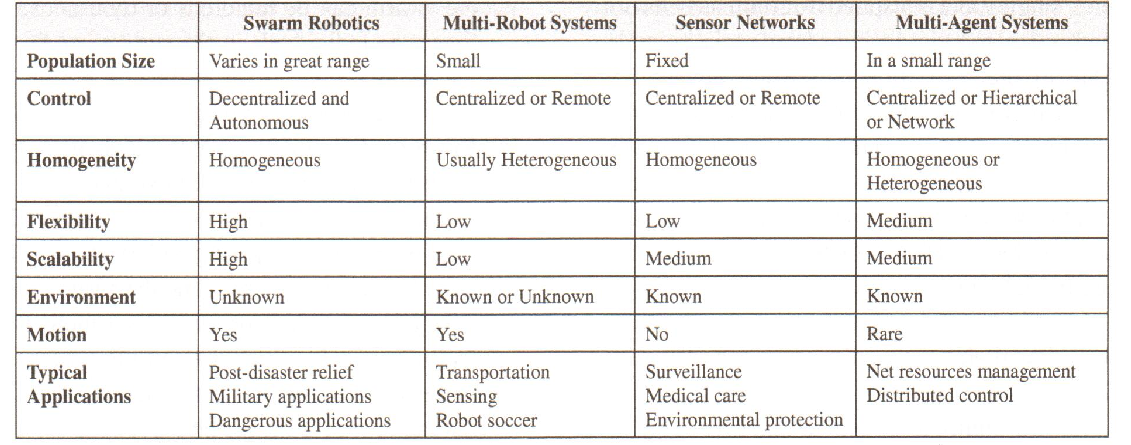
\includegraphics[width=\textwidth]
		{Resources/PNG/vergleich-mrs-swarmrobotic.png}
	\caption{Vergleich der Unterschiedlichen Systeme}
\end{figure}


\section{Ameisenalgorithmen}
\subsection{Optimaler Weg bei futtersbeschaffenden Ameisen}
\paragraph{Funktionsweise}
\begin{itemize}
	\item Eine Ameise verlässt den Bau, das nest (N) und sucht Futter auf einem
		\textbf{zufälligen Weg}
	\item Es gibt mehrere Zweige zur Futterquelle
	\item Weg wird mit \textbf{Pheromon}, einer chemischen Substanz markiert.
	\item Findet die Ameise Futter, schleppt sie das Futter auf dem gleichen oder
		einem anderen Weg zurück, der Weg wird dabei ev. ein weiteres Mal markiert.
	\item Weitere Ameisen, die zur Futtersuche starten, \textbf{orientieren sich}
		bei der Futtersuche \textbf{an den Pheromonspuren}
	\item Ameisen folgen \textbf{bevorzugt}, aber nicht immer den markierten Wegen
	\item Auf langen Wegen ist die Ameisendichte wegen der größeren Entfernung
		geringer, das Phero\-mon verdunstet schneller.
	\item Wenn ein Ausreißer einen kürzeren Weg findet und einige andere Ameisen
		beginnen diesem Weg zu folgen, wird die Ameisendichte auf dem längerenWeg
		immer geringer und der kürzere Weg setzt sich durch
\end{itemize}
\begin{figure}[H]
	\begin{center}
		\includegraphics[scale=0.6]{Resources/PNG/AmeisenAlgorithmus.PNG}
		\caption{Darstellung des Ameisenalgorithmus Prinzips}
		\label{fig:PNG/AmeisenAlgorithmus.PNG}
	\end{center}
\end{figure}

\pagebreak

\subsection{Ant Colony Optimization Algorithm (ACO)}
\paragraph{Kategorien}
\begin{description}
	\item[Tourenplanung (Routing):] Travelling Salesman Problem
	\item[Zuordnung (Assignment):] optimale Zuordnung von Personen oder
		Betriebsmitteln auf Stellen oder Aufgaben
	\item[Ablaufplanung (Scheduling):] Verteilung von knappen Ressourcen auf
		Prozesse die zeitlich begrenzt sind
	\item[Teilmengen Problem (Subset):] aus einer Menge von Objekten muss eine
		Teilmenge gefunden werden, damit eine vorgegebene Bedingung erfüllt und
		eine Zielfunktion optimiert wird.
\end{description}

\paragraph{Eigenschaften}
\begin{itemize}
	\item optimaler Weg ist der \textbf{kürzeste Weg} zwischen zwei Punkten
	\item \textbf{globale Information}: Belegung mit künstlichen Pheromonen als zentrale Idee
	\item Wahrscheinlichkeits-gestützte, \textbf{lokale Entscheidungen} - Ameise erkennt unmittelbare Nachbarschaft
\end{itemize}

\paragraph{Funktionsweise}
\begin{enumerate}
	\item Ameisen laufen entlang des Graphen
	\item Eine Ameise erzeugt eine Lösung gemäß lokaler Information und Pheromon
	\item Update beinhaltet neu aufgetragene Pheromone und Verdunstung
		vorhandener Pheromone
	\item Operationen, die globales Wissen vorraussetzen und damit nicht von
		einzelnen Ameisen bewerkstelligt werden können
\end{enumerate}
\begin{itemize}
	\item Diskretisierung der Zeit t: in einem Zeitschritt erzeugen alle Ameisen
		eine vollständige Lösung.
	\item Eine \textbf{Pheromon-Matrix} enthält die  Intensität der Pheromone
		$T_ij(t)$ enthält die Intensität der Pheromone auf einer Kante vom Knoten
		$i$ zum Knoten $j$ im Graphen
	\item Eine Matrix für lokale Informationen enthält die Sichtbarkeit der Stadt
		(d.h. die jeweils reziproke Distanz): $n_ij = \dfrac{1 }{d_ij}$
\end{itemize}

\subsection{Traveling Salesman Problem}
\begin{itemize}
	\item Vorhanden: \textbf{vollständiger gerichteter Graph}
	\item Gesucht: \textbf{Rundtour durch alle Städte}
\end{itemize}
Ameisen laufen durch den Graphen, die Kolonie ermittelt den Optimalen Weg.
Es erweist sich als vorteilhaft, für jede Ameise eine andere zufällig gewählte
Stadt als Ausgangspunkt für die Tour zu nehmen.

\begin{figure}[H]
	\begin{center}
		\includegraphics[scale=0.5]{Resources/PNG/ACO.PNG}
		\caption{Ameisenalgorithmus - Schritte}
		\label{fig:PNG/ACO.PNG}
	\end{center}
\end{figure}

\paragraph{Entscheidung für nächste Stadt}
\begin{itemize}
	\item Jede Ameise besitzt eine Liste mit gültiger Nachbarschaft $N$
	\item Die Entscheidung in einem Knoten bzgl. der nächsten Stadt fällt gemäß
		folgender Formel:
		$$
			p_{i j}^k=\left\{
				\begin{array}{ll}
					\frac {
							\left[\tau_{i j}(t)\right]^\alpha \cdot
							\left[\eta_{i j}\right]^\beta
						} {
							\sum_{l \in J_k^k}
							\left[\tau_{i l}(t)\right]^\alpha \cdot
							\left[\eta_{i l}\right]^\beta
						} & \text{ für } j \in J_i^k \\
					0 & \text{ für } j \notin J_i^k
				\end{array}
			\right.
		$$
	\item $\alpha$ und $\beta$ steuern das Verhältnis zwischen Anteil der
		Pheromone und lokaler Information
	\item für $\alpha$ hat man den klassischen Greedy Ansatz
\end{itemize}
